\chapter{Economic Analysis}

\section{Acetic anhydride production}

	To demonstrate how to evaluate the economic attributes of a chemical process, we use the production of acetic anhydride from acetone. We are going to follow the book of \cite{AlMalah2016}. The process flowsheet for acetic anhydride production is made of PFR with a recycle for the unreacted acetone, followed by two downstream separation units: rectifying and distillation column and finally the conversion of ketene and acetic acid into acetic anhydride using CSTR. The flowsheet is presented on figure \ref{fig:Acetic_Flowsheet}
	
	\begin{figure}[h!]
		\centering
		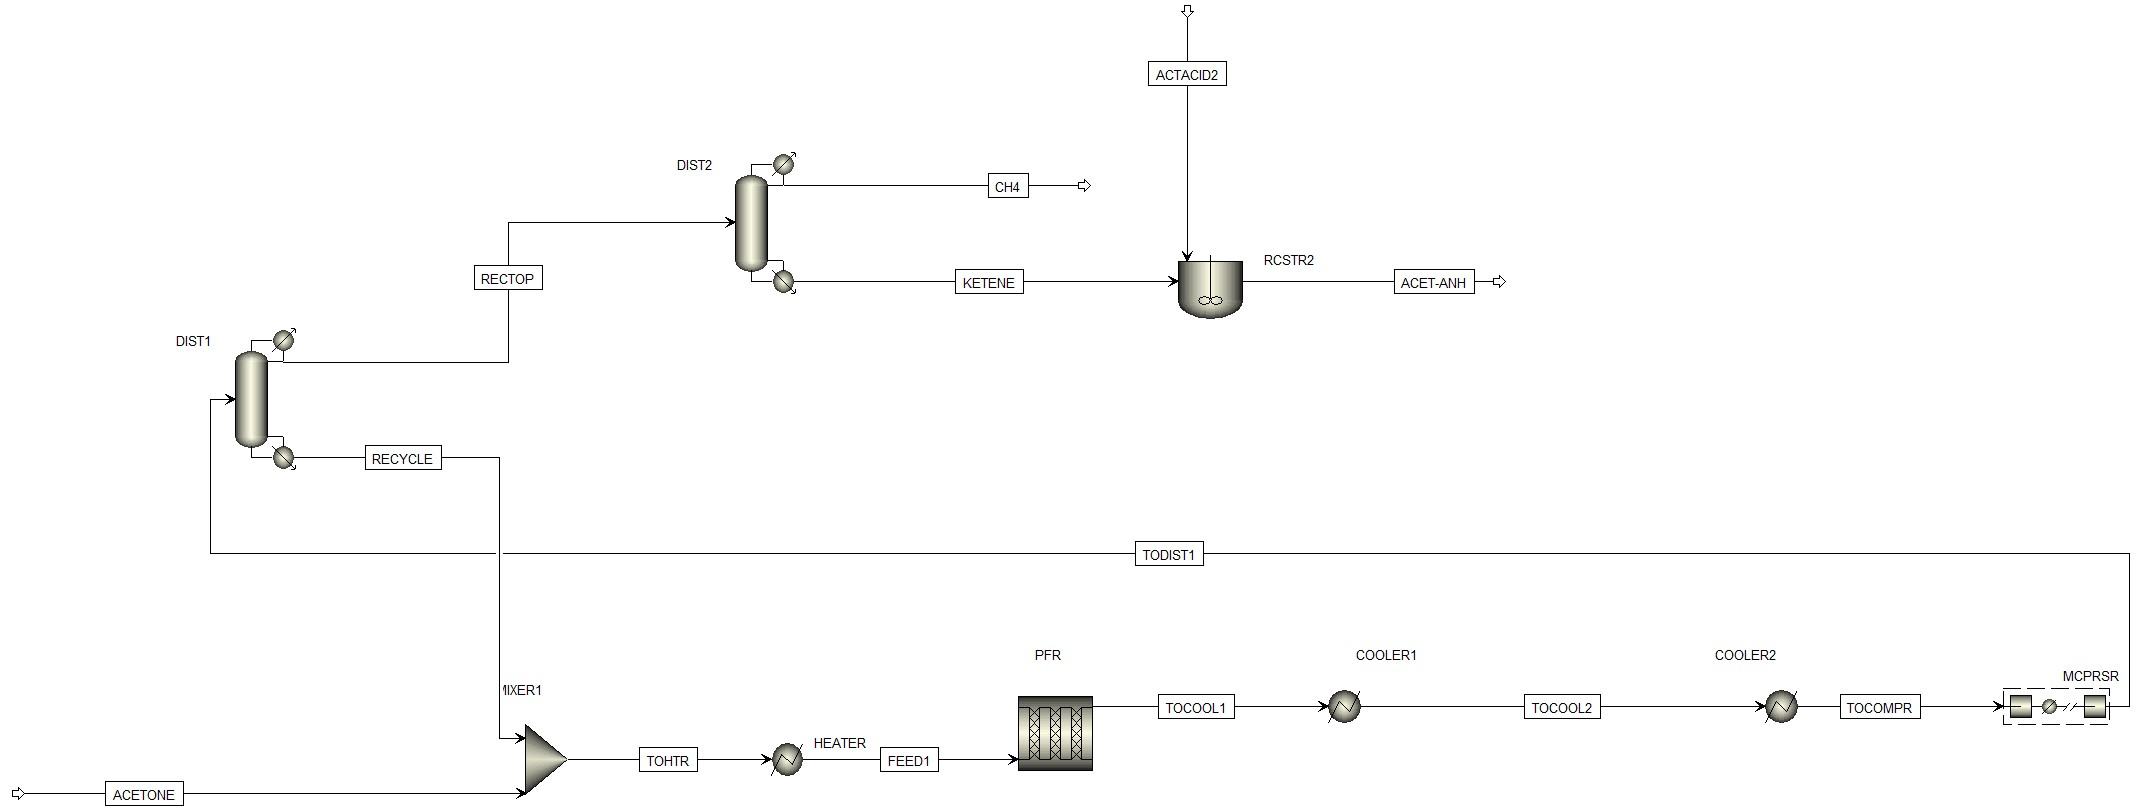
\includegraphics[trim= 0cm 0cm 0cm 0cm,clip,width=\textwidth]{Cost_estimation/Figures/Flowsheet.jpg}
		\caption{The process flowsheet for acetic anhydride production with recycling of the unreacted acetone}
		\label{fig:Acetic_Flowsheet}
	\end{figure}

	The methods recommended by Aspen for Carboxylic Acids are activity coefficient methods with Nothangel or Hayden-O'Connel model with vapour phase association with NRTL-HOC or WILSON-NTH. In this simulation, Wilson-NTH is chosen. 
	
	All the missing binary interaction coefficients can be estimated by the UNIFAC method, which uses information about the structure of particular components to predict its behaviour. 
	
	The reactor design in Aspen Plus depends on the reactor type the user chooses. In this exercise, the PFR and CSTR reactors are used. The first reactor is PFR. Firstly, one needs to decide on the reactor type. The adiabatic reactor is used in this case. Then the reactor dimensions should be provided. The third step is to define the kinetics of the reaction need to be defined. The powerlow model is used. Kinetic data can be found in \cite{Fogler1974}. 
	
	Due to the fact that the outlet stream from the reactor contains a high amount of unreacted acetone, which should be separated and recirculated. This can be done with an absorption column or distillation column. 
	
	Although, the vapour feed to the column should be compressed before the separation. The 4-stage compressor can be used for that purpose. 
	Then the stream is fed into the column. This is an example of a rare process, which belongs to the cryogenic group due to the very lower temperature in the condenser. The acetone is a bottom product and is recycled. In the second column, the methane is separated from ketene in a distillation column. 
	The ketene is a bottom product of the distillation and is used as a feed for the CSTR reactor. The ketene is mixed with acetic acid in the reactor. First, the information about working conditions (T and P) and the reactor's technical details (Volume) must be introduced to Aspen Plus. Then the reaction is described. The powerlaw model is used again, but this time the reaction type is "equilibrium", meaning that the Gibbs energy minimization algorithm is used. 
	
	The input file can be found at the end of this chapter. The results of the simulation are presented in table \ref{tab:Acet_Simu_Result_Basic}:
	
	\begin{table}[h!]
		\adjustbox{max width=\textwidth}{%
		\begin{tabular}{ll|lllllllllllll}
			& Units   & ACET-ANH & ACETONE  & ACTACID2 & CH4       & FEED1    & KETENE   & RECTOP    & RECYCLE  & TOCOMPR  & TOCOOL1  & TOCOOL2  & TODIST1  & TOHTR   \\ \hline
			Temperature    & C       & 7.50E+01 & 2.50E+01 & 2.50E+01 & -9.79E+01 & 7.62E+02 & 5.59E+01 & -6.05E+01 & 2.03E+02 & 9.00E+01 & 6.28E+02 & 1.40E+02 & 1.95E+02 & 7.01E+01 \\
			Pressure       & bar     & 1.50E+01 & 1.60E+00 & 1.50E+01 & 2.80E+01  & 1.60E+00 & 2.80E+01 & 2.90E+01  & 2.90E+01 & 1.60E+00 & 1.60E+00 & 1.60E+00 & 2.90E+01 & 1.60E+00 \\ \hline
			Mole Flows     & kmol/hr & 1.72E+01 & 1.72E+01 & 1.71E+01 & 1.72E+01  & 7.37E+01 & 1.72E+01 & 3.44E+01  & 5.65E+01 & 9.09E+01 & 9.09E+01 & 9.09E+01 & 9.09E+01 & 7.37E+01 \\
			$CH_3COH_3$        & kmol/hr & 1.22E-02 & 1.72E+01 & 0.00E+00 & 4.92E-32  & 7.37E+01 & 1.22E-02 & 1.22E-02  & 5.65E+01 & 5.65E+01 & 5.65E+01 & 5.65E+01 & 5.65E+01 & 7.37E+01 \\
			$C_2H_2O$          & kmol/hr & 7.94E-02 & 0.00E+00 & 0.00E+00 & 2.82E-14  & 1.22E-02 & 1.72E+01 & 1.72E+01  & 1.22E-02 & 1.72E+01 & 1.72E+01 & 1.72E+01 & 1.72E+01 & 1.22E-02 \\
			$CH_4$            & kmol/hr & 1.72E-02 & 0.00E+00 & 0.00E+00 & 1.72E+01  & 1.72E-12 & 1.72E-02 & 1.72E+01  & 1.72E-12 & 1.72E+01 & 1.72E+01 & 1.72E+01 & 1.72E+01 & 1.72E-12 \\
			$CH_3COOH$        & kmol/hr & 1.16E-05 & 0.00E+00 & 1.71E+01 & 0.00E+00  & 0.00E+00 & 0.00E+00 & 0.00E+00  & 0.00E+00 & 0.00E+00 & 0.00E+00 & 0.00E+00 & 0.00E+00 & 0.00E+00 \\
			ACET-ANH       & kmol/hr & 1.71E+01 & 0.00E+00 & 0.00E+00 & 0.00E+00  & 0.00E+00 & 0.00E+00 & 0.00E+00  & 0.00E+00 & 0.00E+00 & 0.00E+00 & 0.00E+00 & 0.00E+00 & 0.00E+00 \\
			$H_2O$          & kmol/hr & 0.00E+00 & 0.00E+00 & 0.00E+00 & 0.00E+00  & 0.00E+00 & 0.00E+00 & 0.00E+00  & 0.00E+00 & 0.00E+00 & 0.00E+00 & 0.00E+00 & 0.00E+00 & 0.00E+00 \\ \hline
			Mole Fractions &         &          &          &          &           &          &          &           &          &          &          &          &          &          \\
			$CH_3COH_3$        &         & 7.08E-04 & 1.00E+00 & 0.00E+00 & 2.86E-33  & 1.00E+00 & 7.08E-04 & 3.54E-04  & 1.00E+00 & 6.21E-01 & 6.21E-01 & 6.21E-01 & 6.21E-01 & 1.00E+00 \\
			$C_2H_2O$          &         & 4.61E-03 & 0.00E+00 & 0.00E+00 & 1.64E-15  & 1.66E-04 & 9.98E-01 & 5.00E-01  & 2.16E-04 & 1.89E-01 & 1.89E-01 & 1.89E-01 & 1.89E-01 & 1.66E-04 \\
			$CH_4$            &         & 9.98E-04 & 0.00E+00 & 0.00E+00 & 1.00E+00  & 2.33E-14 & 9.98E-04 & 5.00E-01  & 3.04E-14 & 1.89E-01 & 1.89E-01 & 1.89E-01 & 1.89E-01 & 2.33E-14 \\
			$CH_3COOH$        &         & 6.76E-07 & 0.00E+00 & 1.00E+00 & 0.00E+00  & 0.00E+00 & 0.00E+00 & 0.00E+00  & 0.00E+00 & 0.00E+00 & 0.00E+00 & 0.00E+00 & 0.00E+00 & 0.00E+00 \\
			ACET-ANH       &         & 9.94E-01 & 0.00E+00 & 0.00E+00 & 0.00E+00  & 0.00E+00 & 0.00E+00 & 0.00E+00  & 0.00E+00 & 0.00E+00 & 0.00E+00 & 0.00E+00 & 0.00E+00 & 0.00E+00 \\
			$H_2O$          &         & 0.00E+00 & 0.00E+00 & 0.00E+00 & 0.00E+00  & 0.00E+00 & 0.00E+00 & 0.00E+00  & 0.00E+00 & 0.00E+00 & 0.00E+00 & 0.00E+00 & 0.00E+00 & 0.00E+00
		\end{tabular} }
	\caption{Simulation result of the acetic anhydride production}
	\label{tab:Acet_Simu_Result_Basic}
	\end{table}

	If we have the process simulation ready and stable, we can move to the economic analysis of the process. The economic analysis requires defining feed and product stream prices, and defining utilities in terms of pricing and associating them with pieces of equipment, such as a pump, compressor, condenser, reboiler, and heater. The economic analysis consists of several steps.
	
	\begin{enumerate}[label=\textbf{Step \arabic{enumi}}:,ref=Step \arabic{enumi}]
		
	\item Investment options
	
	In "Navigation" panel, let us go to "Setup" | "Costing Options" | "Costing options" tab form to specify "operating life of plant", "length of plant startup" and "start of basic engineering". %The figure \ref{fig:Investment_Aspen_Plus} shows the "costing option" window. 
	
%	\begin{figure}[h!]
%		\centering
%		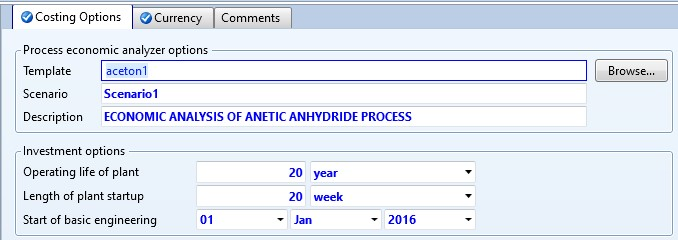
\includegraphics[trim= 0cm 0cm 0cm 0cm,clip,width=0.5\textwidth]{Cost_estimation/Figures/Investment_options_Aspen_Plus.jpg}
%		\caption{Investment options}
%		\label{fig:Investment_Aspen_Plus}
%	\end{figure}

	\item Feed, product and utility prices
	
	In the "Setup" | "Stream Price" | "Input" form, the price per unit of the feed or product stream can be specified. In the "Utilities" folder, each utility used in the simulation is characterized. If pre-defined utility is used, then it has its own "purchase price" or "energy price". The price of a utility can be modified by entering detail information of the that utility. The price used in this exercise are shown in table \ref{tab:Stream_prices} and the utility prices have default values suggested by the software.
	
	\begin{table}[!ht]
		\centering
		\begin{tabular}{|l|l|l|l|l|l|l|l|l|l|}
			\hline
			Stream ID & Source & Destination & Basis & Price & Unit \\ \hline
			ACET-ANH & RCSTR2 & ~ & Mass & 1000 & \$/tonne  \\ \hline
			ACTACID2 & ~ & RCSTR2 & Mass & 600 & \$/tonne   \\ \hline
			ACETONE & ~ & MIXER1 & Mass & 1200 & \$/tonne  \\ \hline
			CH4 & DIST2 & ~ & Mass & 6150 & \$/tonne   \\ \hline
		\end{tabular}
	\caption{Feed and product prices}
	\label{tab:Stream_prices}
	\end{table}
	
	\item Activation of the economic module
	
	There are two routs to perform economic analysis with Aspen environment. First one is to use the economic module, which is incorporated in the Aspen Plus software. The second one is to use stand-alone module called "Aspen Economic Analyzer" (APEA). We are going to focus on the second method as it is more comprehensive and give more flexibility. 
	
	Nevertheless which method is used, the general steps are the same: "Mapping", "Sizing" (\ref{ste:Mapping}) and "Evaluation" (\ref{ste:ProjectEvaluation}). Details on each step will be covered in the following text.
	
	The first step is to send the process simulation to the APEA. It can be done with "Send to APEA" button in the "Economics". Next, a new project needs to be created. Then the simulation data can be loaded, but special attention needs to be paid to check if correct fluid are associated to each utility. In this case, "AIR" utility should associated with air fluid, "FH100" utility with high-temperature hot oil, and "REFRIG4" with refrigerant	ethane.
	
	The details of the economic variables can be found in the "Project Basis View". The list of equipment is located in the "Process View" section. In case of need, more pieces of equipment can be added in this section directly (so it is not needed to go back to the process simulation).
	
	\item Mapping and sizing \label{ste:Mapping}
	
	The "Map option" can be activated with the "Map simulator Items" button located at the top of the page. The "Size equipment" should be marked, while "Custom sizing" can be left unmarked. "Customize sizing" option allows to interfere with the details of equipment sizing. In the "Map Preview" window all the flowsheet objects are mapped with APEA built-in objects. We are going to used the following mapping:
	
	\begin{enumerate}
		\item COOLER1 is "Floating head shell and tube exchanger" because of significant temperature difference between the hot and cold stream.
		\item COOLER2 is "Air cooler" to reflect the fact that “AIR” utility is used.
		\item DST1(RADFRAC) and DST2(RADFRAC); The distillation columns consist the sets of equipment, and each of the should be specify.
		\begin{itemize}
			\item Tower type is "Multiple diameter, trayed or packed tower".
			\item Condenser type is "Bare pipe immersion coil".
			\item Condenser drum is "Horizontal drum".
			\item Reflux pump type is "Centrifugal single or multi-stage pump".
		\end{itemize}
		\item Heater type is "Box type process furnace".
		\item Mixer can be represented as "Agitated tank – enclosed".
		\item The compressor type is “Centrifugal compressor - horizontal".
		\item PFR is "Packed tower".
		\item CSTR is "Agitated tank – enclosed, jacketed".
	\end{enumerate}

	The mapping and sizing are performed automatically. It 
	
	\item Debugging 
	
	The next step would be to performed the project evaluation by click on the "Evaluate Project" button. If things go smooth then you will reach the final executive summary for costs without hassles and you can go to the \ref{ste:ProjectEvaluation}. However, you may get warning or error messages during the evaluation step regarding sizing or missing input data of some pieces of equipment. f you look at the generated report, you will find that APEA reports an error, which is due	to improper entry, such as the type of material of construction or a property value that is out of range. On the other hand, the warning message alarms the user that there might be an error incurred in the user’s selected mapped object specifications.
	
	\begin{itemize}
		\item HEATER
		
		\textit{ERROR> 'FU -    5' STRESS FOR MATERIAL A 214   IS ZERO AT A TEMPERATURE OF  791.85 SYSTEM MAY NOT CONTAIN STRESS VALUES FOR THE MATERIAL.}
		
		This means that material of construction A214 (Carbon Steel) is not suitable for a high-temperature heater. The default Carbon steel A214 can be replaced with S347.
		
		Each piece of equipment can be modified in the "Project View" section. Right click on an item and select modify to access the details of each equipment. After change the inner "Evaluate" button can be used evaluate only the selected item. \\
		
		\item PFR
		
		\textit{Component Item Description: PFR
			User Tag Number: PFR
			*Component Ref \#: 2
			WARN > 'TW -    2' PACKING TYPE '      ' AND/OR VOLUME INCORRECT.}
		
		If we use "1.0 CRR Ceramic raschig ring" as the "Packing type". \\
		
		\item COOLER 1
		
		\textit{Component Item Description: COOLER1
			User Tag Number: COOLER1
			*Component Ref \#: 17
			WARN > 'HE -   17' DESIGN TEMPERATURE TOO HIGH FOR VACUUM OR EXTERNAL PRESSURE DESIGN}
		
		COOLER1 material can be specified as “347S” and “SS347” for construction for both tube and shell.
		
	\end{itemize}
	
	\item Project evaluation \label{ste:ProjectEvaluation}
	
	Clicking on "Capital Costs" o generate a full-fledge report s that include all cost-based technical project details, including design, equipment, civil, structural, piping, mechanical, steel, instrumental, electrical, insulation, paint, labor, management, and the project metrics, such as Independent Project Analysis (IPA) metrics and Project Evaluation System (PES) summary and cost check. 
	
	The investment analysis of the project is summarized in table \ref{tab:AceticInvestment}.
	
	\begin{table}[H]
		\centering
		\adjustbox{max width=\textwidth}{%
		\begin{tabular}{l|ll}
			ITEM                                                               & UNITS          &               \\ \hline
			&                &               \\
			TW    (Number of Weeks per Period)                                 & Weeks/period   & 52            \\
			T    (Number of Periods for Analysis)                              & Period         & 20            \\
			DTEPC    (Duration of EPC Phase)                                   & Period         & 0.75          \\
			DT    (Duration of EPC Phase and Startup)                          & Period         & 1.13462       \\
			WORKP    (Working Capital Percentage)                              & Percent/period & 5             \\
			OPCHG    (Operating Charges)                                       & Percent/period & 25            \\
			PLANTOVH    (Plant Overhead)                                       & Percent/period & 50            \\
			CAPT    (Total Project Cost)                                       & Cost           & 1.35E+07      \\
			RAWT    (Total Raw Material Cost)                                  & Cost/period    & 1.45E+07      \\
			PRODT    (Total Product Sales)                                     & Cost/period    & 2.76E+07      \\
			OPMT    (Total Operating Labor and Maintenance Cost)               & Cost/period    & 1.36E+06      \\
			UTILT    (Total Utilities Cost)                                    & Cost/period    & 547531        \\
			ROR    (Desired Rate of Return/Interest Rate)                      & Percent/period & 20            \\
			AF    (ROR Annuity Factor)                                         &                & 5             \\
			TAXR    (Tax Rate)                                                 & Percent/period & 40            \\
			IF    (ROR Interest Factor)                                        &                & 1.2           \\
			ECONLIFE    (Economic Life of Project)                             & Period         & 10            \\
			SALVAL    (Salvage Value (Percent of Initial Capital Cost))        & Percent        & 20            \\
			DEPMETH    (Depreciation Method)                                   &                & Straight Line \\
			DEPMETHN    (Depreciation Method Id)                               &                & 1             \\
			ESCAP    (Project Capital Escalation)                              & Percent/period & 5             \\
			ESPROD    (Products Escalation)                                    & Percent/period & 5             \\
			ESRAW    (Raw Material Escalation)                                 & Percent/period & 3.5           \\
			ESLAB    (Operating and Maintenance Labor Escalation)              & Percent/period & 3             \\
			ESUT    (Utilities Escalation)                                     & Percent/period & 3             \\
			START    (Start Period for Plant Startup)                          & Period         & 1             \\
			PODE    (Desired Payout Period (excluding EPC and Startup Phases)) & Period         &               \\
			POD    (Desired Payout Period)                                     & Period         &               \\
			DESRET    (Desired Return on Project for Sales Forecasting)        & Percent/Period & 10.5          \\
			END    (End Period for Economic Life of Project)                   & Period         & 10            \\
			GA    (G and A Expenses)                                           & Percent/Period & 8             \\
			DTEP    (Duration of EP Phase before Start of Construction)        & Period         & 0.480769      \\
			OP    (Total Operating Labor Cost)                                 & Cost/period    & 1.24E+06      \\
			MT    (Total Maintenance Cost)                                     & Cost/period    & 115000       \\ \hline
		\end{tabular} }
	\caption{Summery of the investment analysis}
	\label{tab:AceticInvestment}
	\end{table}
		
	The summery of the overall cost obtained from the economic analysis can be found in table \ref{tab:AceticProdInvestment}.
	
	\begin{table}[H]
		\centering
		\begin{tabular}{l|ll}
			INVESTMENT:                &  \\ \hline
			Currency Conversion Rate   & 1.00                                               & USD/U.S. DOLLAR                                        \\
			Total Project Capital Cost & 13'450'400.00                                        & USD                                                    \\
			Total Operating Cost       & 18'820'400.00                                        & USD/Year                                               \\
			Total Raw Materials Cost   & 14'536'300.00                                        & USD/Year                                               \\
			Total Utilities Cost       & 547'531.00                                          & USD/Year                                               \\
			Total Product Sales        & 27'587'800.00                                        & USD/Year                                               \\
			Desired Rate of Return     & 20.00                                              & Percent/'Year                                          \\
			P.O. Period                & 5.83                                               & Year            \\ \hline                                      
		\end{tabular}
	\caption{Overall costs of the acetic anhydride production}
	\label{tab:AceticProdInvestment}
	\end{table}

	\hrule
	Remember that total operating cost includes:
	
	\begin{multicols}{2}
		\begin{itemize}
			\item Total raw materials cost
			\item Total utilities cost
			\item Operating labor cost
			\item Maintenance cost
			\item Operating charges
			\item Plant overhead
			\item Subtotal operating cost
			\item General and admin cost
		\end{itemize} 
	\end{multicols}
	\hrule 
	
	\item Investment analysis 
	
	An economy of an arbitrary process can be analysed based on different indicators. The most popular indicator is the \textbf{Net Present Value (NPV)}, which applies to a series of cash flows occurring at different times and accounts for the "time value of money". NPV is determined by calculating the costs (negative cash flows) and benefits (positive cash flows) for each period of an investment. After the cash flow for each period is calculated, the present value (PV) of each one is achieved by discounting its future value (see equation \ref{EQ:PV}) at a periodic rate of return (the rate of return dictated by the market). NPV is the sum of all the discounted future cash flows, as given by equation \ref{EQ:NPV}.
	
	\begin{equation}
		PV = \cfrac{R_t}{(1+r)^t}
		\label{EQ:PV}
	\end{equation}

	\begin{equation}
		NPV = \sum_{i=0}^{N} \cfrac{R_{t}}{(1+i)^t} = \sum_{i=0}^{N} PV
		\label{EQ:NPV}
	\end{equation}

	where $t$ is the time of the cash flow, $r$ is the discount rate, i.e. the return that could be earned per unit of time on an investment with similar risk and $R_{t}$ is the net cash flow i.e. cash inflow – cash outflow, at time $t$ and $N$ is the number of time intervals.
	
	Based on the project evaluation performed in \ref{ste:ProjectEvaluation}, the PV and NPV are found. The PV and NPV curves are presented on figure \ref{fig:CashFlow}.
	
	\begin{figure}[h!]
		\centering
		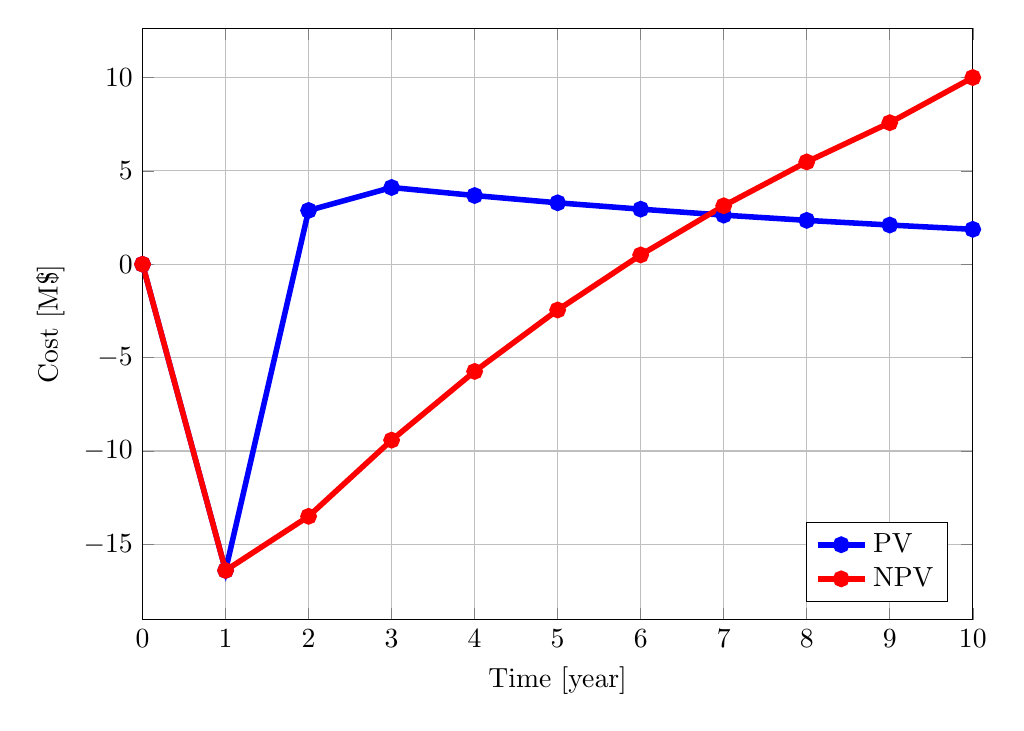
\begin{tikzpicture}
			\begin{axis}[
				xmin=0, xmax=10,
				grid = both,
				major grid style = {lightgray},
				minor grid style = {lightgray!25},
				width = \textwidth,
				height = 0.75\textwidth,
				legend cell align = {left},
				legend pos = south east,
				xlabel={Time~[year]},
				ylabel={Cost~[M\$]}
				]
				
				\addplot[line width=2pt,blue, mark = *]
				coordinates {
					(0,0)	(1,-1.64E+01)	(2,2.88E+00)	(3,4.11E+00)	(4,3.68E+00)	(5,3.29E+00)	(6,2.95E+00)	(7,2.63E+00)	(8,2.35E+00)	(9,2.10E+00)	(10,1.87E+00)
				};
				
				\addplot[line width=2pt,red, mark = *]
				coordinates {
					(0,0)	(1,-1.64E+01)	(2,-1.35E+01)	(3,-9.42E+00)	(4,-5.74E+00)	(5,-2.45E+00)	(6,0.498682E+00)	(7,3.13E+00)	(8,5.48E+00)	(9,7.58E+00)	(10,1.00E+01)
				};
				
				\legend{
					PV, 
					NPV
				}
				
			\end{axis}
			
		\end{tikzpicture}
	\caption{Cash flow}
	\label{fig:CashFlow}
	\end{figure}

	NPV is negative for the first 6 years and becomes positive after that, which means that the project appears to be profitable, from year seven onward.
	
	The second indicator is the \textbf{discounted payout period (DPP)}, which is described by equation \ref{EQ:DPP}
	
	{\footnotesize
	\begin{equation}
		DPP = \text{Years with negative NPV} + \cfrac{\text{|NPV|}}{\text{PV}} = 5 + \cfrac{|-2.45E+06|}{2.95E+06} = 5.83~\text{years}
		\label{EQ:DPP}
	\end{equation} }

	DPP	represents the length of time required to recover the cost of an investment. The payout (or, payback) period of a given investment project is an important determinant of whether to undertake the project, as longer payback periods are typically not desirable for investment projects. Notice that the payout period indicator ignores any benefits that occur after the payback period and, therefore, does not measure profitability. In addition, it ignores the time value of money.
	
	The third indicator is the \textbf{profitability index (PI)} that shows the present value of the benefits relative to the present value	of the costs. The PI is defined as given by equation \ref{EQ:PI}
	
	\begin{equation}
		PI = \cfrac{\text{Present Value of the Cumulative Cash Inflows (PVI)}}{\text{Present Value of the Cumulative Cash Outflows (PVO)}}
		\label{EQ:PI}
	\end{equation}
	
	If the profitability index is greater than one, then the project appears to be profitable. If this index is less than one, then the project appears not to be profitable. If this number equals one then the project incurs no losses or gains (break-even point). The time evolution of PI is shown on figure \ref{fig:PI}.
	
	\begin{figure}[h!]
		\centering
		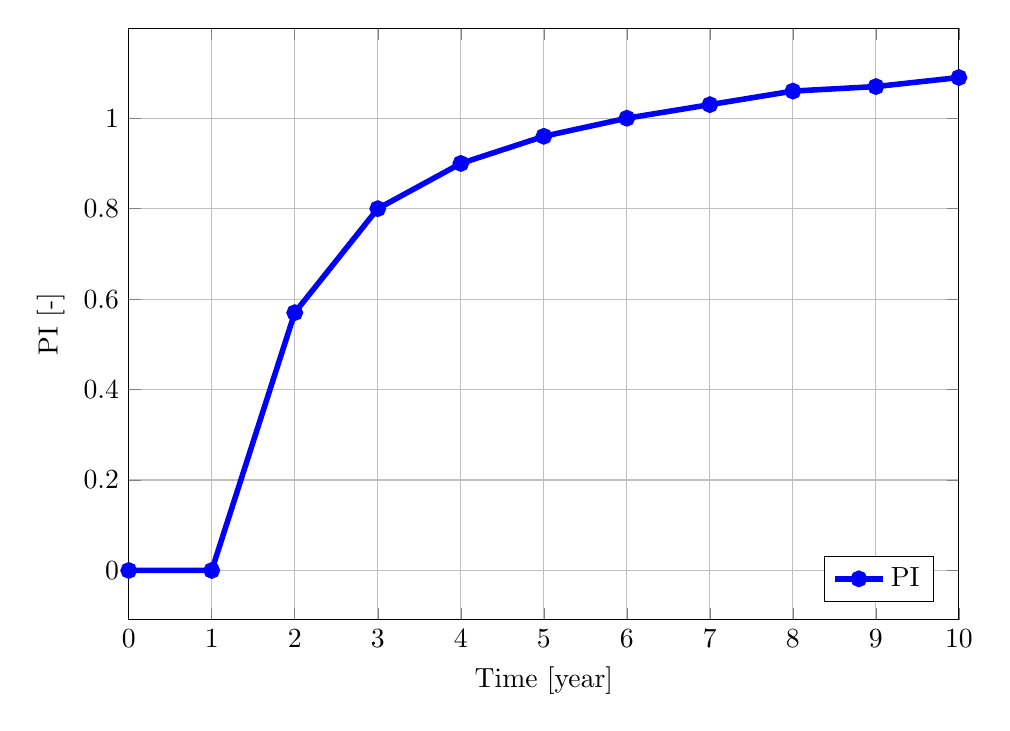
\begin{tikzpicture}
			\begin{axis}[
				xmin=0, xmax=10,
				grid = both,
				major grid style = {lightgray},
				minor grid style = {lightgray!25},
				width = \textwidth,
				height = 0.75\textwidth,
				legend cell align = {left},
				legend pos = south east,
				xlabel={Time~[year]},
				ylabel={PI~[-]}
				]
				
				\addplot[line width=2pt,blue, mark = *]
				coordinates { (0,0)	(1,0)	(2,0.57)	(3,0.80)	(4,0.9)	(5,0.96)	(6,1.00)	(7,1.03)	(8,1.06)	(9,1.07)	(10,1.09)
				};
				
				\legend{
					PI
				}
				
			\end{axis}
			
		\end{tikzpicture}
		\caption{Profitability index}
		\label{fig:PI}
	\end{figure}

	The fourth indicator is the \textbf{internal rate of return (IRR}). Iternal rate of return (IRR) is the discount rate at which the net present value of an investment becomes zero. In more specific terms, the IRR of an investment is the discount rate at	which the net present value of costs (negative cash flows) of the investment equals the net present value of the benefits (positive cash flows) of the investment. In this case, the $IRR = 34.27\%$. A project should only be accepted if its IRR is NOT less than the target internal rate of return. When comparing two or more mutually exclusive projects, the project with the highest value of IRR should be considered.
	
	The fifth indicator is the \textbf{modified internal rate of return (MIRR)}. IRR assumes that positive cash flows are reinvested at the same rate of return as that of the investment (i.e., the project which generates them). This assumption is questionable as funds are reinvested at a rate that reflects the organization’s cost of capital or return on cash. Consequently, if we stick with the assumption of equal rate for both negative and positive cash flow, then IRR gives an optimistic (i.e., overestimated) rate of return for the cash flows. In addition, for projects with alternating positive and negative cash flows, more than one IRR may be found, which may lead to confusion. To use MIRR, two interest rates are needed: The reinvestment rate for the positive cash flow (PV) and the finance rate for the negative cash flow (NV). The MIRR is given by equation \ref{EQ:MIRR}.
	
	\begin{equation}
		MIRR(\%) = \left[ \left[ \cfrac{FV}{-PV} \right]^{\cfrac{1}{EPELP}} -1 \right] \times 100\%
		\label{EQ:MIRR}
	\end{equation}

	where $EPELP$ is the "End Period for Economic Life of Project" (i.e., $EPELP=10$ years, by default), $PV$ is the sum of cash flows (brought to the beginning of the first period), and $FV$ is the sum of positive cash flows (brought to the end of the last period).
	
	The MIRR value was found to be $21.03\%$, which is less than IRR.

\end{enumerate}
	
	\clearpage
%	\VerbatimInput{Input.txt}
	
	